\chapter{O coração e o ciclo cardíaco}\label{ch:b2:heart}

Retire o \omterm{def:b2:heart:anatomy}{coração} de uma rã e coloque-o numa solução salina, e ele
continua batendo durante horas --- sem nervos, sem encéfalo, sem \omterm{def:b2:blood-circulation:blood}{sangue},
apenas um músculo que se contrai sozinho cerca de uma vez por segundo
porque um pequeno grupo de suas células não consegue ficar parado. Um
\omterm{def:b2:heart:anatomy}{coração} humano faz isso uns três bilhões de vezes ao longo de uma vida,
movendo da ordem de duzentos milhões de litros, sem nunca ser
desligado. Este capítulo trata dessa bomba: suas câmaras e valvas, o
ciclo de enchimento e esvaziamento e as pressões que o impulsionam, o
sistema elétrico que o marca e o traçado que ele deixa na pele, a lei
que lhe permite ajustar seu débito ao que recebe, batimento a
batimento, e os nervos e hormônios que ajustam seu ritmo e sua força.

\section{A bomba}

\begin{definition}[Câmaras e valvas]\label{def:b2:heart:anatomy}
\index{coração}\index{átrio}\index{ventrículo}\index{valva cardíaca}
O coração é formado por duas bombas lado a lado, cada uma com um
\emph{átrio}, que recebe o \omterm{def:b2:blood-circulation:blood}{sangue} das \omterm{def:b2:blood-circulation:vessels}{veias}, e um \emph{ventrículo},
que o ejeta numa \omterm{def:b2:blood-circulation:vessels}{artéria}. O coração direito recebe o \omterm{def:b2:blood-circulation:blood}{sangue} das \omterm{def:b2:blood-circulation:vessels}{veias}
cavas e o envia aos pulmões pela \omterm{def:b2:blood-circulation:vessels}{artéria} pulmonar; o coração esquerdo o
recebe de volta das \omterm{def:b2:blood-circulation:vessels}{veias} pulmonares e o envia ao corpo pela aorta.
Quatro valvas tornam o fluxo unidirecional: as \emph{valvas
atrioventriculares} (tricúspide à direita, mitral à esquerda),
válvulas presas por cordas aos músculos papilares, de modo que não
possam ser empurradas de volta para o átrio; e as \emph{valvas
semilunares} (pulmonar e aórtica), três bolsas que se enchem e se
fecham quando a pressão arterial supera a do ventrículo. As valvas são
passivas: abrem-se e fecham-se apenas por diferenças de pressão. A
parede ventricular é o \emph{miocárdio}, músculo estriado de células
ramificadas unidas pelas extremidades por \emph{discos intercalares}
repletos de junções comunicantes, de modo que o ventrículo inteiro é
eletricamente uma única célula e se contrai como uma só; a parede do
ventrículo esquerdo é três vezes mais espessa que a do direito porque
bombeia contra uma pressão cinco vezes maior. O músculo cardíaco é
nutrido por suas próprias \emph{\omterm{def:b2:blood-circulation:vessels}{artérias} coronárias}, que se enchem na
diástole, e funciona quase inteiramente por metabolismo aeróbio --- ele
não pode contrair dívidas.
\end{definition}

\begin{omfigure}
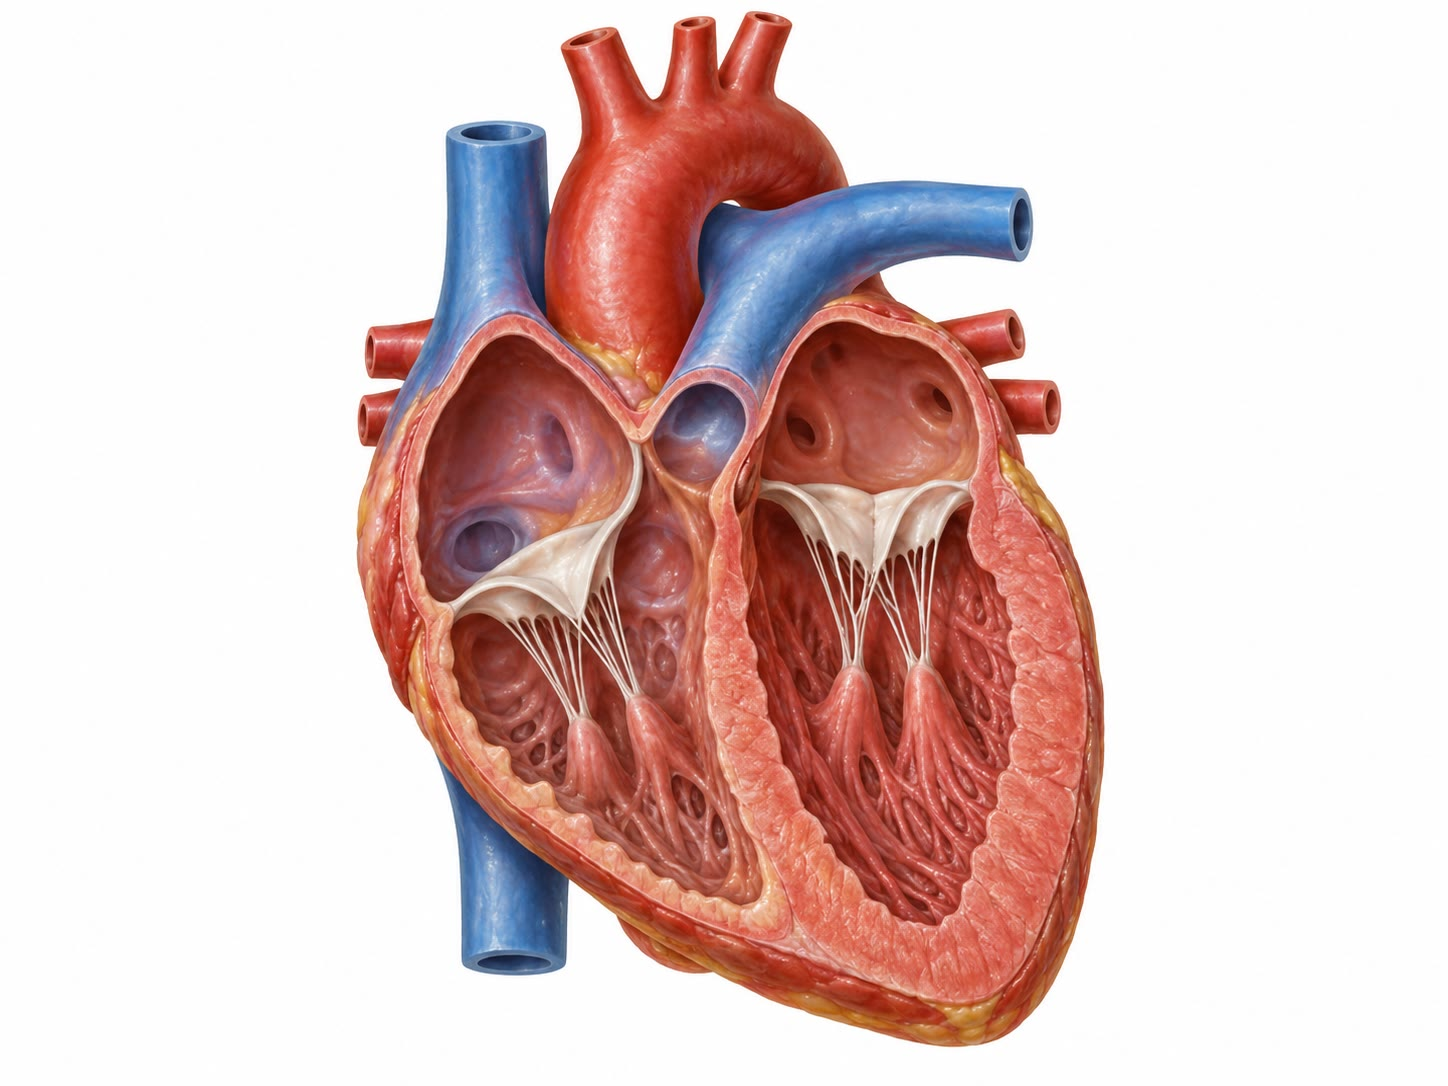
\includegraphics[width=0.55\linewidth]{images/book4/ai/b4-17-heart-cutaway.jpg}

{\small O \omterm{def:b2:heart:anatomy}{coração} em corte frontal: dois \omterm{def:b2:heart:anatomy}{átrios} em cima, dois
\omterm{def:b2:heart:anatomy}{ventrículos} embaixo, o espesso \omterm{def:b2:heart:anatomy}{ventrículo} esquerdo, as valvas
atrioventriculares com suas cordas e as duas grandes \omterm{def:b2:blood-circulation:vessels}{artérias} saindo
pelo topo.}
\end{omfigure}

\begin{proposition}[O ciclo cardíaco]\label{prop:b2:heart:cycle}
\index{ciclo cardíaco}\index{sístole}\index{diástole}\index{volume sistólico}\index{fração de ejeção}
Um batimento em repouso dura cerca de \qty{0.8}{s}. \emph{Diástole}
(\qty{0.5}{s}): os \omterm{def:b2:heart:anatomy}{ventrículos} relaxam, sua pressão cai abaixo da dos
\omterm{def:b2:heart:anatomy}{átrios}, as valvas atrioventriculares se abrem e o \omterm{def:b2:blood-circulation:blood}{sangue} entra, em
grande parte passivamente, depois com um impulso final da contração
atrial; o \omterm{def:b2:heart:anatomy}{ventrículo} termina a diástole com cerca de \qty{120}{mL} (o
\emph{volume diastólico final}). \emph{Sístole} (\qty{0.3}{s}): os
\omterm{def:b2:heart:anatomy}{ventrículos} se contraem; assim que sua pressão supera a pressão
atrial, as valvas atrioventriculares se fecham (a primeira bulha
cardíaca, ``tum''), e durante alguns centésimos de segundo o \omterm{def:b2:heart:anatomy}{ventrículo}
comprime uma câmara fechada --- a \emph{contração isovolumétrica} ---
até que sua pressão ultrapasse a pressão arterial (\qty{80}{mmHg} à
esquerda), quando as valvas semilunares se abrem e o \omterm{def:b2:blood-circulation:blood}{sangue} é ejetado.
O \omterm{def:b2:heart:anatomy}{ventrículo} esquerdo chega a \qty{120}{mmHg} e expele cerca de
\qty{70}{mL} (o \emph{\omterm{prop:b2:heart:cycle}{volume sistólico}}, uma \emph{\omterm{prop:b2:heart:cycle}{fração de ejeção}}
de \qty{60}{\%}); ao relaxar, sua pressão cai abaixo da aórtica, a
valva aórtica se fecha bruscamente (a segunda bulha, ``tá''), e um
relaxamento isovolumétrico leva a pressão até o nível atrial, quando o
enchimento recomeça. O \omterm{def:b2:heart:anatomy}{coração} direito faz o mesmo a um quinto da
pressão, ejetando o mesmo volume.
\end{proposition}

\begin{omfigure}
\begin{tikzpicture}
\begin{axis}[
  width=0.9\linewidth, height=7.2cm,
  axis x line=bottom, axis y line=left,
  xmin=0, xmax=0.8, ymin=0, ymax=130,
  xlabel={tempo no ciclo (s)}, ylabel={pressão (\unit{mmHg})},
  xlabel style={font=\small, at={(axis description cs:0.5,-0.1)}, anchor=north},
  ylabel style={font=\small},
  tick label style={font=\small}, xtick={0,0.1,0.3,0.8}, ytick={0,40,80,120},
  legend style={font=\scriptsize, at={(0.6,0.45)}, anchor=west, draw=none},
  clip=false,
]
% aortic pressure
\addplot[very thick, omThm] coordinates {(0,82) (0.05,80) (0.1,80) (0.12,95) (0.16,115) (0.2,120) (0.25,112) (0.3,100) (0.32,104) (0.34,100) (0.45,94) (0.6,88) (0.8,82)};
\addlegendentry{aorta}
% left ventricular pressure
\addplot[very thick, omDef] coordinates {(0,5) (0.04,8) (0.05,10) (0.08,60) (0.1,80) (0.12,95) (0.16,115) (0.2,120) (0.25,112) (0.3,100) (0.32,60) (0.35,20) (0.38,5) (0.5,3) (0.7,5) (0.75,8) (0.8,5)};
\addlegendentry{ventrículo esquerdo}
% atrial pressure
\addplot[thick, omProp] coordinates {(0,6) (0.03,9) (0.06,6) (0.1,8) (0.15,6) (0.3,7) (0.36,10) (0.4,5) (0.6,6) (0.75,9) (0.8,6)};
\addlegendentry{átrio esquerdo}
\draw[dashed, gray] (axis cs:0.05,0) -- (axis cs:0.05,128); \node[font=\scriptsize, anchor=south, align=center] at (axis cs:0.05,128) {mitral\\fecha};
\draw[dashed, gray] (axis cs:0.1,0) -- (axis cs:0.1,128); \node[font=\scriptsize, anchor=south, align=center] at (axis cs:0.13,128) {aórtica\\abre};
\draw[dashed, gray] (axis cs:0.31,0) -- (axis cs:0.31,128); \node[font=\scriptsize, anchor=south, align=center] at (axis cs:0.31,128) {aórtica\\fecha};
\draw[dashed, gray] (axis cs:0.38,0) -- (axis cs:0.38,128); \node[font=\scriptsize, anchor=south, align=center] at (axis cs:0.4,128) {mitral\\abre};
\node[font=\scriptsize] at (axis cs:0.2,45) {sístole};
\node[font=\scriptsize] at (axis cs:0.55,25) {diástole};
\end{axis}
\end{tikzpicture}

{\small As pressões no \omterm{def:b2:heart:anatomy}{coração} esquerdo durante um batimento. O
\omterm{def:b2:heart:anatomy}{ventrículo} comprime uma câmara fechada até superar a pressão aórtica,
ejeta enquanto permanece acima dela, relaxa até cair abaixo da pressão
atrial e se enche.}
\end{omfigure}

\begin{theorem}[O trabalho do coração]\label{thm:b2:heart:work}
\index{trabalho cardíaco}\index{alça pressão--volume}
Representado como pressão em função do volume, um batimento do
\omterm{def:b2:heart:anatomy}{ventrículo} esquerdo descreve uma alça --- enchimento ao longo da parte
inferior, contração isovolumétrica subindo pelo lado direito, ejeção ao
longo do topo, de \qty{120}{mL} a \qty{50}{mL}, relaxamento
isovolumétrico descendo pelo lado esquerdo ---, e a área da alça é o
trabalho mecânico do batimento:
\[
W = \oint P\,\mathrm{d}V \approx \bar P_{\text{ejeção}}\times \text{volume sistólico} \approx \qty{100}{mmHg}\times\qty{70}{mL} = \qty{0.93}{J}.
\]
A 72 batimentos por minuto, o \omterm{def:b2:heart:anatomy}{ventrículo} esquerdo produz cerca de
\qty{1.1}{W}, e o direito \qty{0.2}{W}; o metabolismo do \omterm{def:b2:heart:anatomy}{coração} é de
uns \qty{8}{W}, de modo que sua eficiência mecânica é de cerca de
\qty{15}{\%}, sendo o restante calor e o custo da tensão. Elevar a
pressão contra a qual o \omterm{def:b2:heart:anatomy}{coração} bombeia (hipertensão, uma valva aórtica
estreitada) eleva o trabalho por batimento na mesma proporção, e o
músculo se espessa em resposta, como qualquer músculo --- até que sua
irrigação coronária já não acompanhe seu volume.
\end{theorem}
\begin{proof}
Trabalho é força vezes distância e, para uma pressão que age sobre uma
parede em movimento, pressão vezes volume varrido:
$\mathrm{d}W = P\,\mathrm{d}V$. Ao longo de uma alça fechada, o
trabalho líquido é a área delimitada (o enchimento a baixa pressão custa
pouco; a ejeção a alta pressão devolve muito mais).
$\qty{100}{mmHg} = \qty{1.33e4}{Pa}$ e $\qty{70}{mL} =
\qty{7e-5}{m^3}$: $1.33\times 10^{4}\times 7\times 10^{-5} =
\qty{0.93}{J}$; vezes $1.2$ batimento por segundo, \qty{1.1}{W}.
\end{proof}

\begin{omfigure}
\begin{tikzpicture}
\begin{axis}[
  width=0.62\linewidth, height=6cm,
  axis x line=bottom, axis y line=left,
  xmin=0, xmax=150, ymin=0, ymax=140,
  xlabel={volume do ventrículo esquerdo (\unit{mL})}, ylabel={pressão (\unit{mmHg})},
  xlabel style={font=\small, at={(axis description cs:0.5,-0.12)}, anchor=north},
  ylabel style={font=\small},
  tick label style={font=\small}, xtick={0,50,120}, ytick={0,80,120},
  clip=false,
]
\fill[omDef!12] (axis cs:50,5) -- (axis cs:120,8) -- (axis cs:120,80) -- (axis cs:110,115) -- (axis cs:80,122) -- (axis cs:50,100) -- cycle;
\draw[very thick, omDef, ->] (axis cs:50,5) -- (axis cs:120,8);
\draw[very thick, omDef, ->] (axis cs:120,8) -- (axis cs:120,80);
\draw[very thick, omDef, ->] (axis cs:120,80) .. controls (axis cs:110,118) and (axis cs:80,125) .. (axis cs:50,100);
\draw[very thick, omDef, ->] (axis cs:50,100) -- (axis cs:50,5);
\node[font=\scriptsize, anchor=south] at (axis cs:85,11) {enchimento};
\node[font=\scriptsize, anchor=west] at (axis cs:122,44) {contração isovolumétrica};
\node[font=\scriptsize, anchor=south] at (axis cs:85,124) {ejeção};
\node[font=\scriptsize, anchor=east] at (axis cs:48,52) {relaxamento};
\node[font=\scriptsize] at (axis cs:85,60) {área $=$ trabalho, \qty{0.9}{J}};
\end{axis}
\end{tikzpicture}

{\small A \omterm{thm:b2:heart:work}{alça pressão--volume} do \omterm{def:b2:heart:anatomy}{ventrículo} esquerdo. A área delimitada
é o trabalho de um batimento; uma pressão arterial mais alta eleva o
topo da alça e, com ele, o trabalho.}
\end{omfigure}

\section{O relógio próprio do coração}

\begin{proposition}[Automatismo e condução]\label{prop:b2:heart:conduction}
\index{nó sinoatrial}\index{marca-passo}\index{nó atrioventricular}\index{fibras de Purkinje}
O batimento se origina no \emph{\omterm{prop:b2:heart:conduction}{nó sinoatrial}}, um grupo de células
musculares especializadas na parede do \omterm{def:b2:heart:anatomy}{átrio} direito cujo potencial de
membrana nunca repousa: após cada potencial de ação, ele sobe
lentamente (um \emph{potencial marca-passo}, produzido por uma corrente
de sódio que se ativa em potenciais negativos e por canais de cálcio)
até atingir o limiar e disparar de novo, cerca de cem vezes por minuto
se deixado por conta própria. O impulso se propaga pelo músculo
atrial, de célula em célula através das junções comunicantes, e os
\omterm{def:b2:heart:anatomy}{átrios} se contraem; ele chega ao \emph{\omterm{prop:b2:heart:conduction}{nó atrioventricular}}, a única
ponte elétrica entre \omterm{def:b2:heart:anatomy}{átrios} e \omterm{def:b2:heart:anatomy}{ventrículos}, que conduz devagar e o
atrasa um décimo de segundo --- tempo para que os \omterm{def:b2:heart:anatomy}{átrios} terminem de
encher os \omterm{def:b2:heart:anatomy}{ventrículos}; depois ele desce rapidamente pelo \emph{feixe
de His} e pelas \emph{\omterm{prop:b2:heart:conduction}{fibras de Purkinje}}, células de condução rápida
que o levam a todo o músculo ventricular em \qty{30}{ms}, de modo que
os \omterm{def:b2:heart:anatomy}{ventrículos} se contraem do ápice para cima, como uma unidade, e
impulsionam o \omterm{def:b2:blood-circulation:blood}{sangue} em direção às valvas de saída. Cada parte desse
sistema consegue marcar o ritmo sozinha, cada uma mais lentamente que a
anterior (o nó a 100, o nó AV a 50, as \omterm{prop:b2:heart:conduction}{fibras de Purkinje} a 30), de
modo que, se o nó falhar, um centro inferior assume --- num ritmo mais
lento.
\end{proposition}
\begin{proof}[Evidências]
Um \omterm{def:b2:heart:anatomy}{coração} isolado, ou uma tira de tecido sinoatrial, bate numa placa
sem nervos; uma tira de \omterm{def:b2:heart:anatomy}{ventrículo} também bate, porém mais devagar.
Esfriar ou aquecer apenas o \omterm{prop:b2:heart:conduction}{nó sinoatrial} muda o ritmo do \omterm{def:b2:heart:anatomy}{coração}
inteiro; seccionar o feixe AV dissocia os \omterm{def:b2:heart:anatomy}{ventrículos}, que passam a
bater em seu próprio ritmo lento enquanto os \omterm{def:b2:heart:anatomy}{átrios} continuam no ritmo
do nó (bloqueio cardíaco). O registro de uma única célula do nó mostra
a despolarização diastólica lenta que nenhuma célula muscular comum
tem; bloquear a corrente marca-passo a desacelera.
\end{proof}

\begin{omfigure}
\begin{tikzpicture}[every node/.style={font=\scriptsize}, >=stealth]
  % simplified heart outline, scaled up
  \draw[thick, fill=omThm!6] (0,0) .. controls (-4.2,1.3) and (-3.8,5.4) .. (-1.3,5.8) .. controls (0,6.1) and (0.6,5.6) .. (1.3,5.8) .. controls (3.8,5.4) and (4.2,1.3) .. (0,0);
  \draw[thick] (-3.0,3.5) .. controls (-0.8,3.85) and (0.8,3.85) .. (3.0,3.5);
  \draw[thick] (0,3.75) -- (0,0.6);
  \node at (-1.5,4.7) {átrio direito}; \node at (1.5,4.7) {átrio esquerdo};
  \node[align=center] at (-1.3,2.55) {ventrículo\\direito}; \node[align=center] at (1.3,2.55) {ventrículo\\esquerdo};
  % SA node
  \fill[omDef] (-2.5,5.0) circle (0.16); \node[omDef, anchor=east] at (-3.3,5.4) {nó SA}; \draw[omDef] (-3.3,5.35) -- (-2.62,5.08);
  \draw[omDef, dashed] (-2.5,5.0) circle (0.45); \draw[omDef, dashed] (-2.5,5.0) circle (0.8);
  % AV node
  \fill[omDef] (-0.25,3.7) circle (0.14); \node[omDef, anchor=west] at (0.15,4.05) {nó AV}; \draw[omDef] (0.15,4.05) -- (-0.12,3.78);
  % bundle and Purkinje
  \draw[very thick, omDef] (-0.25,3.6) -- (-0.25,2.1);
  \draw[very thick, omDef] (-0.25,2.1) .. controls (-0.8,1.4) .. (-1.9,1.1);
  \draw[very thick, omDef] (-0.25,2.1) .. controls (0.8,1.4) .. (1.9,1.1);
  \foreach \p in {(-1.9,1.1),(1.9,1.1)} { \draw[omDef] \p -- ++(-0.3,0.6); \draw[omDef] \p -- ++(0.3,0.7); \draw[omDef] \p -- ++(0,0.85); }
  \node[omDef, anchor=west] at (3.4,1.0) {fibras de Purkinje}; \draw[omDef] (3.4,1.0) -- (2.2,1.1);
  \node[omDef, anchor=east] at (-0.45,3.05) {feixe de His};
  % timing
  \node[anchor=west, align=left] at (5.6,5.0) {o nó SA dispara: $t = 0$\\despolarização dos átrios: 0--\qty{80}{ms}};
  \node[anchor=west, align=left] at (5.6,3.5) {atraso no nó AV: \qty{100}{ms}};
  \node[anchor=west, align=left] at (5.6,1.9) {feixe e fibras de Purkinje:\\ventrículos despolarizados\\até \qty{220}{ms}, ápice primeiro};
\end{tikzpicture}

{\small O sistema de condução. O \omterm{prop:b2:heart:conduction}{nó sinoatrial} dispara, os \omterm{def:b2:heart:anatomy}{átrios} se
despolarizam, o \omterm{prop:b2:heart:conduction}{nó atrioventricular} atrasa o impulso, e o feixe e as
\omterm{prop:b2:heart:conduction}{fibras de Purkinje} o levam aos \omterm{def:b2:heart:anatomy}{ventrículos}, do ápice para cima.}
\end{omfigure}

\begin{proposition}[O eletrocardiograma]\label{prop:b2:heart:ecg}
\index{eletrocardiograma}
O \omterm{def:b2:heart:anatomy}{coração} é uma grande massa de células que se despolarizam e se
repolarizam em sequência, e as correntes que circulam no corpo em torno
dele podem ser registradas como tensões de um milivolt entre eletrodos
colocados nos membros: é o \emph{eletrocardiograma}. Suas ondas são os
eventos do sistema de condução: a \emph{onda P} é a despolarização
atrial; o \emph{intervalo PR}, plano (\qty{0.16}{s}), é o atraso AV; o
\emph{complexo QRS}, agudo e breve (\qty{0.08}{s}), é a despolarização
ventricular --- grande porque a massa ventricular é grande, breve porque
as \omterm{prop:b2:heart:conduction}{fibras de Purkinje} são rápidas; a \emph{onda T} é a repolarização
ventricular. (A repolarização atrial fica escondida no QRS.) O traçado
informa o momento e a condução, e não a força: um nó AV bloqueado
alonga o intervalo PR ou dissocia a onda P do QRS, uma região morta do
\omterm{def:b2:heart:anatomy}{ventrículo} deforma o QRS, um \omterm{def:b2:heart:anatomy}{átrio} irregular (fibrilação atrial)
substitui as ondas P por ruído e faz os \omterm{def:b2:heart:anatomy}{ventrículos} baterem de modo
irregular, e o intervalo entre as ondas R dá a frequência.
\end{proposition}

\begin{omfigure}
\begin{tikzpicture}
\begin{axis}[
  width=0.9\linewidth, height=5.2cm,
  axis x line=bottom, axis y line=left,
  xmin=0, xmax=1.0, ymin=-0.4, ymax=1.3,
  xlabel={tempo (s)}, ylabel={mV},
  xlabel style={font=\small, at={(axis description cs:0.5,-0.12)}, anchor=north},
  ylabel style={font=\small},
  tick label style={font=\small}, xtick={0,0.2,0.4,0.6,0.8,1.0}, ytick={0,1},
  clip=false,
]
\addplot[very thick, omDef] coordinates {(0,0) (0.08,0) (0.1,0.05) (0.14,0.15) (0.18,0.05) (0.2,0) (0.28,0) (0.3,-0.1) (0.31,0) (0.33,1.1) (0.35,0) (0.36,-0.25) (0.375,0) (0.5,0) (0.54,0.1) (0.58,0.28) (0.62,0.1) (0.65,0) (0.88,0) (0.9,0.05) (0.94,0.15) (0.98,0.05) (1.0,0)};
\node[font=\scriptsize, anchor=south] at (axis cs:0.14,0.17) {P};
\node[font=\scriptsize, anchor=south] at (axis cs:0.33,1.12) {R};
\node[font=\scriptsize, anchor=north] at (axis cs:0.295,-0.11) {Q};
\node[font=\scriptsize, anchor=north] at (axis cs:0.365,-0.27) {S};
\node[font=\scriptsize, anchor=south] at (axis cs:0.58,0.3) {T};
\draw[<->, gray] (axis cs:0.1,0.45) -- (axis cs:0.3,0.45); \node[font=\scriptsize, anchor=south, gray] at (axis cs:0.2,0.46) {PR \qty{0.16}{s}};
\draw[<->, gray] (axis cs:0.3,0.6) -- (axis cs:0.375,0.6); \node[font=\scriptsize, anchor=west, gray] at (axis cs:0.38,0.6) {QRS \qty{0.08}{s}};
\draw[<->, gray] (axis cs:0.33,1.25) -- (axis cs:0.94,1.25); \node[font=\scriptsize, anchor=south, gray] at (axis cs:0.63,1.25) {intervalo R--R $=$ 60/frequência};
\end{axis}
\end{tikzpicture}

{\small Um eletrocardiograma normal: P (\omterm{def:b2:heart:anatomy}{átrios}), o atraso PR no nó AV,
QRS (despolarização ventricular), T (repolarização ventricular).}
\end{omfigure}

\section{A regulação do débito}

\begin{theorem}[A lei de Frank--Starling]\label{thm:b2:heart:starling}
\index{lei de Frank--Starling}\index{pré-carga}\index{débito cardíaco}
A força de uma contração ventricular aumenta com o volume que encheu o
\omterm{def:b2:heart:anatomy}{ventrículo}: dentro da faixa de funcionamento, quanto mais o \omterm{def:b2:heart:anatomy}{ventrículo} é
distendido na diástole (a \emph{pré-carga}), mais ele ejeta na sístole.
O \omterm{def:b2:heart:anatomy}{coração} bombeia, portanto, batimento a batimento, tudo o que recebe
--- um aumento de \qty{20}{\%} do retorno venoso é respondido por um
aumento de \qty{20}{\%} do \omterm{prop:b2:heart:cycle}{volume sistólico} sem nenhum nervo nem
hormônio ---, e os dois \omterm{def:b2:heart:anatomy}{ventrículos}, que precisam mover o mesmo volume,
se equilibram automaticamente: se o \omterm{def:b2:heart:anatomy}{coração} direito envia mais \omterm{def:b2:blood-circulation:blood}{sangue}
aos pulmões, o \omterm{def:b2:heart:anatomy}{coração} esquerdo recebe mais e bombeia mais. O mecanismo
está no \omterm{def:b2:cell-differentiation:fibre}{sarcômero}: nos comprimentos curtos de um \omterm{def:b2:heart:anatomy}{ventrículo} pouco cheio,
os filamentos grossos e finos se sobrepõem demais e a sensibilidade ao
cálcio é baixa; a distensão em direção ao comprimento ótimo
(\qty{2.2}{\micro m}) aumenta tanto a sobreposição disponível para as
pontes cruzadas quanto a sensibilidade, de modo que o mesmo pulso de
cálcio produz mais força. Além do ótimo (um \omterm{def:b2:heart:anatomy}{coração} superdistendido,
em insuficiência), a força volta a cair.
\end{theorem}
\begin{proof}[Evidências]
Frank (1895) registrou a pressão desenvolvida por um \omterm{def:b2:heart:anatomy}{ventrículo} de rã
cheio com diferentes volumes: a pressão de pico subia com o volume de
enchimento até um máximo e depois caía. Starling (1914), com uma
preparação coração--pulmão de cão em que o retorno venoso e a
resistência arterial podiam ser fixados de modo independente, mostrou
que aumentar o retorno aumentava o débito batimento a batimento, e que
um aumento da resistência arterial era respondido, após alguns
batimentos de acúmulo, por um volume diastólico final maior e um débito
restaurado --- o \omterm{def:b2:heart:anatomy}{ventrículo} responde a uma carga distendendo-se e a uma
distensão contraindo-se com mais força.
\end{proof}

\begin{omfigure}
\begin{tikzpicture}
\begin{axis}[
  width=0.66\linewidth, height=5.4cm,
  axis x line=bottom, axis y line=left,
  xmin=0, xmax=200, ymin=0, ymax=140,
  xlabel={volume diastólico final (\unit{mL})}, ylabel={volume sistólico (\unit{mL})},
  xlabel style={font=\small, at={(axis description cs:0.5,-0.13)}, anchor=north},
  ylabel style={font=\small},
  tick label style={font=\small}, xtick={0,50,100,150,200}, ytick={0,50,100},
  legend style={font=\scriptsize, at={(0.5,-0.3)}, anchor=north, draw=none, legend columns=3},
  clip=false,
]
\addplot[very thick, omDef, domain=40:200, samples=60] {130*(1-exp(-(x-40)/70))};
\addlegendentry{normal}
\addplot[very thick, omThm, domain=40:200, samples=60] {130*1.3*(1-exp(-(x-40)/55))};
\addlegendentry{com estimulação simpática}
\addplot[very thick, omExo!70!black, domain=40:200, samples=60] {130*0.5*(1-exp(-(x-40)/90))};
\addlegendentry{coração em insuficiência}
\fill[omDef] (axis cs:120,88) circle (2pt); \node[font=\scriptsize, anchor=south east] at (axis cs:118,90) {repouso};
\end{axis}
\end{tikzpicture}

{\small Curvas de Starling. O \omterm{prop:b2:heart:cycle}{volume sistólico} aumenta com o
enchimento; os nervos simpáticos deslocam a curva para cima (mais débito
com o mesmo enchimento), e um \omterm{def:b2:heart:anatomy}{coração} em insuficiência a desloca para
baixo.}
\end{omfigure}

\begin{proposition}[Nervos e hormônios]\label{prop:b2:heart:control}
\index{sistema nervoso simpático!coração}\index{nervo vago}\index{adrenalina}\index{débito cardíaco}
O \omterm{thm:b2:heart:starling}{débito cardíaco} é a frequência cardíaca vezes o \omterm{prop:b2:heart:cycle}{volume sistólico},
\qty{5}{L/min} em repouso e até \qty{25}{L/min} no exercício de um
atleta treinado. Os dois fatores são fixados pelos nervos autônomos. O
\emph{vago} (parassimpático), liberando acetilcolina sobre o \omterm{prop:b2:heart:conduction}{nó
sinoatrial}, desacelera a subida do potencial marca-passo e mantém a
frequência de repouso em 70, e não nos 100 próprios do nó; secione os
vagos e a frequência sobe. Os nervos \emph{simpáticos}, liberando
noradrenalina, e a medula suprarrenal, liberando \emph{adrenalina} no
\omterm{def:b2:blood-circulation:blood}{sangue}, aceleram essa subida (mais batimentos), aceleram a condução e
elevam a força de contração para qualquer enchimento (uma curva de
Starling mais íngreme, a propriedade chamada \emph{contratilidade}),
aumentando o cálcio fornecido aos \omterm{def:b2:cell-differentiation:fibre}{sarcômeros} a cada batimento. No
exercício, o freio vagal é liberado primeiro, depois o acelerador
simpático é acionado, e uma frequência de 180 com um \omterm{prop:b2:heart:cycle}{volume sistólico} de
\qty{140}{mL} dá \qty{25}{L/min}; os sinais passam pelos receptores e
segundos mensageiros do \cref{ch:b2:cell-signalling}, e o conjunto é comandado pelos
centros reguladores da pressão do \cref{ch:b2:blood-pressure}.
\end{proposition}

\begin{example}[Ler um coração]\label{ex:b2:heart:reading}
Duas bulhas por batimento: tum, as valvas AV se fechando no início da
sístole; tá, as valvas semilunares se fechando no fim. Um sopro é o
escoamento turbulento através de uma valva estreitada (uma estenose)
ou de volta através de uma valva que vaza (uma insuficiência): um sopro
entre o tum e o tá é uma valva mitral que vaza ou uma valva aórtica
estreitada; depois do tá, uma valva aórtica que vaza. Um pulso de 70
com uma pressão arterial de $120/80$~mmHg significa um \omterm{prop:b2:heart:cycle}{volume sistólico}
perto de \qty{70}{mL}; uma frequência de 40 num atleta é um grande
\omterm{prop:b2:heart:cycle}{volume sistólico} e um forte tônus vagal; uma frequência de 40 com um
intervalo PR que se alonga até que um batimento falhe é um nó AV
doente. A fisiologia deste capítulo é o que um médico ouve com um
estetoscópio em trinta segundos.
\end{example}

\section{Exercícios}

\begin{exercise}[$\star$]\label{exo:b2:heart:1}
Acompanhe uma gota de \omterm{def:b2:blood-circulation:blood}{sangue} da \omterm{def:b2:blood-circulation:vessels}{veia} cava até a aorta, citando em ordem
cada câmara, valva e vaso.
\end{exercise}

\begin{exercise}[$\star$]\label{exo:b2:heart:2}
Dê as fases do \omterm{prop:b2:heart:cycle}{ciclo cardíaco} com o estado de cada valva em cada fase,
e o evento que causa cada uma das duas bulhas cardíacas.
\end{exercise}

\begin{exercise}[$\star$]\label{exo:b2:heart:3}
Cite em ordem as partes do sistema de condução, com o tempo que o
impulso leva para chegar a cada uma e a onda do ECG que cada uma produz.
\end{exercise}

\begin{exercise}[$\star$]\label{exo:b2:heart:4}
Enuncie a \omterm{thm:b2:heart:starling}{lei de Frank--Starling} e diga por que ela garante que os dois
\omterm{def:b2:heart:anatomy}{ventrículos} bombeiem o mesmo volume.
\end{exercise}

\begin{exercise}[$\star\star$]\label{exo:b2:heart:5}
Um \omterm{def:b2:heart:anatomy}{coração} tem um volume diastólico final de \qty{130}{mL} e um \omterm{prop:b2:heart:cycle}{volume
sistólico} final de \qty{50}{mL} a 70 batimentos por minuto. Calcule o
\omterm{prop:b2:heart:cycle}{volume sistólico}, a \omterm{prop:b2:heart:cycle}{fração de ejeção} e o \omterm{thm:b2:heart:starling}{débito cardíaco}. Um \omterm{def:b2:heart:anatomy}{coração} em
insuficiência tem \qty{180}{mL} e \qty{120}{mL}: refaça o cálculo e diga
o que aconteceu com a \omterm{prop:b2:heart:cycle}{fração de ejeção}.
\end{exercise}

\begin{exercise}[$\star\star$]\label{exo:b2:heart:6}
Calcule o trabalho de um batimento para um \omterm{prop:b2:heart:cycle}{volume sistólico} de
\qty{70}{mL} a uma pressão média de ejeção de \qty{100}{mmHg}, e a
potência a 72 batimentos por minuto. Refaça o cálculo para um
hipertenso a \qty{150}{mmHg}. Quanto oxigênio a mais por minuto o
segundo \omterm{def:b2:heart:anatomy}{coração} precisa, se a eficiência mecânica é de \qty{15}{\%} e
\qty{1}{mL} de oxigênio fornece \qty{20}{J}?
\end{exercise}

\begin{exercise}[$\star\star$]\label{exo:b2:heart:7}
Num ECG, as ondas R estão separadas por \qty{0.5}{s} num registro e por
\qty{1.5}{s} em outro. Dê as frequências cardíacas. Num terceiro, as
ondas P aparecem a cada \qty{0.6}{s} e os complexos QRS a cada
\qty{1.8}{s}, sem relação fixa. O que aconteceu?
\end{exercise}

\begin{exercise}[$\star\star$]\label{exo:b2:heart:8}
O potencial da célula sinoatrial sobe de \qty{-60}{mV} até um limiar de
\qty{-40}{mV} a \qty{25}{mV/s} antes de cada potencial de ação de
\qty{0.15}{s}. Calcule o intervalo entre os batimentos e a frequência.
A acetilcolina reduz a velocidade de subida a \qty{18}{mV/s} e o
potencial de partida a \qty{-65}{mV}; a noradrenalina eleva a velocidade
de subida a \qty{40}{mV/s}. Calcule as duas frequências.
\end{exercise}

\begin{exercise}[$\star\star$]\label{exo:b2:heart:9}
Explique por que o atraso do nó AV é necessário, o que aconteceria com o
débito sem ele, e por que um nó AV lento (um intervalo PR longo) é
inofensivo até certo ponto e perigoso além dele.
\end{exercise}

\begin{exercise}[$\star\star\star$]\label{exo:b2:heart:10}
Um atleta em repouso tem uma frequência de 45 e um débito de
\qty{5}{L/min}; no exercício, uma frequência de 180 e \qty{30}{L/min}.
Calcule os \omterm{prop:b2:heart:cycle}{volumes sistólicos} e diga com o que a curva de Starling e os
nervos simpáticos contribuem cada um. Por que a frequência não pode
ultrapassar de modo útil cerca de 200?
\end{exercise}

\begin{exercise}[$\star\star\star$]\label{exo:b2:heart:11}
Uma valva aórtica estreitada deixa uma abertura de \qty{1}{cm^2} em vez
de \qty{3}{cm^2}. Usando a continuidade, calcule a velocidade do \omterm{def:b2:blood-circulation:blood}{sangue}
ejetado a \qty{250}{mL/s} através de cada uma e, pela equação de
Bernoulli ($\Delta P = \tfrac12\rho v^2$), a pressão que o \omterm{def:b2:heart:anatomy}{ventrículo}
precisa gerar acima da pressão aórtica em cada caso. O que o \omterm{def:b2:heart:anatomy}{ventrículo}
faz a respeito, e qual é o custo final?
\end{exercise}

\begin{exercise}[$\star\star\star$]\label{exo:b2:heart:12}
``O \omterm{def:b2:heart:anatomy}{coração} é uma bomba que se regula sozinha e é apenas ajustada pelo
sistema nervoso.'' Discuta, distinguindo o que o automatismo, a \omterm{thm:b2:heart:starling}{lei de
Frank--Starling} e os nervos autônomos fornecem cada um, e o que um
\omterm{def:b2:heart:anatomy}{coração} transplantado --- que não tem nervos --- consegue e não consegue
fazer.
\end{exercise}

\section{Problema: Um coração sob carga}

\begin{problem}[{Problema de fim de semana --- um coração acompanhado
do repouso ao exercício e à doença: seu ciclo cronometrado, seu trabalho
calculado, seu eletrocardiograma lido, sua resposta de Starling e seu
controle autônomo quantificados, e o custo de uma valva estreitada
estimado, até o débito em repouso e no exercício, o trabalho por
batimento e o gradiente através da estenose}]
\label{pb:b2:heart:1}
Dados: em repouso, frequência de 70, volume diastólico final de
\qty{130}{mL}, \omterm{prop:b2:heart:cycle}{volume sistólico} final de \qty{60}{mL}, pressão média de
ejeção de \qty{100}{mmHg} ($\qty{1}{mmHg} = \qty{133}{Pa}$), pressão
aórtica de $120/80$~mmHg. A sístole dura \qty{0.3}{s} em qualquer
frequência. Marca-passo: subida de \qty{-60}{mV} a \qty{-40}{mV},
potencial de ação de \qty{0.15}{s}. O \omterm{def:b2:heart:anatomy}{coração} consome \qty{20}{J} por
mililitro de oxigênio, com uma eficiência mecânica de \qty{15}{\%}; o
\omterm{def:b2:blood-circulation:blood}{sangue} coronário leva \qty{0.2}{mL} de oxigênio por mililitro, e o
\omterm{def:b2:heart:anatomy}{coração} extrai \qty{70}{\%} dele. Densidade do \omterm{def:b2:blood-circulation:blood}{sangue}:
\qty{1060}{kg/m^3}.

\medskip
\noindent\textbf{Parte I --- O ciclo em repouso.}
\begin{enumerate}
  \item Calcule o \omterm{prop:b2:heart:cycle}{volume sistólico}, a \omterm{prop:b2:heart:cycle}{fração de ejeção} e o \omterm{thm:b2:heart:starling}{débito
        cardíaco}.
  \item Calcule a duração de um ciclo e a da diástole.
  \item Calcule a taxa média de ejeção durante a sístole, em mililitros
        por segundo, e a velocidade média através de uma valva aórtica de
        \qty{3}{cm^2}.
  \item A pressão ventricular sobe a \qty{1500}{mmHg/s} durante a
        contração isovolumétrica, de 10 a \qty{80}{mmHg}. Quanto tempo
        dura essa fase?
  \item Calcule o trabalho de um batimento e a potência mecânica do
        \omterm{def:b2:heart:anatomy}{ventrículo} esquerdo.
  \item Calcule a potência total do \omterm{def:b2:heart:anatomy}{coração} e seu consumo de oxigênio
        (os dois \omterm{def:b2:heart:anatomy}{ventrículos}: considere o direito como um quinto do
        esquerdo).
  \item Calcule o fluxo sanguíneo coronário necessário para fornecer
        esse oxigênio.
\end{enumerate}

\medskip
\noindent\textbf{Parte II --- O marca-passo e o traçado.}
\begin{enumerate}[resume]
  \item Que velocidade de subida (\unit{mV/s}) dá uma frequência de 70?
  \item O vago é seccionado: a frequência passa a 100. Que velocidade de
        subida é essa?
  \item Calcule a velocidade de subida para uma frequência de 180 no
        exercício.
  \item No ECG em repouso, dê o intervalo R--R e diga a que
        correspondem as ondas P, QRS e T.
  \item O intervalo PR é de \qty{0.16}{s} em repouso. Sua duração se
        deve sobretudo ao atraso do nó AV: explique o que esse atraso
        proporciona e por que uma frequência de 180 exige que o nó também
        acelere.
  \item O ECG de um paciente mostra complexos QRS a cada \qty{1.5}{s} e
        ondas P a cada \qty{0.8}{s}, sem relação entre si. Faça o
        diagnóstico, dê a frequência ventricular e diga que tecido está
        comandando o ritmo dos \omterm{def:b2:heart:anatomy}{ventrículos}.
\end{enumerate}

\medskip
\noindent\textbf{Parte III --- O exercício.}
No exercício, a frequência sobe para 180 e os nervos simpáticos elevam a
contratilidade, de modo que o \omterm{prop:b2:heart:cycle}{volume sistólico} final cai para
\qty{30}{mL}; o retorno venoso eleva o volume diastólico final para
\qty{150}{mL}.
\begin{enumerate}[resume]
  \item Calcule o \omterm{prop:b2:heart:cycle}{volume sistólico}, a \omterm{prop:b2:heart:cycle}{fração de ejeção} e o débito.
  \item Calcule a duração da diástole a 180 e explique por que a
        frequência não pode subir muito mais de modo útil.
  \item Calcule a potência do \omterm{def:b2:heart:anatomy}{ventrículo} esquerdo a uma pressão média de
        ejeção de \qty{120}{mmHg}, e o consumo de oxigênio do \omterm{def:b2:heart:anatomy}{coração}.
  \item Calcule o fluxo coronário necessário e compare com o repouso.
        Por que o encurtamento da diástole é um problema para ele?
  \item Sem os nervos simpáticos (um \omterm{def:b2:heart:anatomy}{coração} transplantado), a
        frequência só sobe lentamente, pela adrenalina do \omterm{def:b2:blood-circulation:blood}{sangue}, e a
        contratilidade sobe menos. Preveja o débito no primeiro minuto de
        exercício, usando apenas a lei de Starling com o mesmo
        enchimento.
  \item Atribua o aumento do débito do repouso ao exercício a suas três
        causas (frequência, enchimento, contratilidade), em litros por
        minuto para cada uma.
\end{enumerate}

\medskip
\noindent\textbf{Parte IV --- Uma valva estreitada.}
A valva aórtica se estreita para \qty{1}{cm^2}.
\begin{enumerate}[resume]
  \item Calcule a velocidade de ejeção em repouso através da valva
        estreitada.
  \item Usando a equação de Bernoulli, $\Delta P = \tfrac12\rho v^{2}$,
        calcule a pressão que o \omterm{def:b2:heart:anatomy}{ventrículo} precisa acrescentar para
        empurrar o \omterm{def:b2:blood-circulation:blood}{sangue} através dela, em mmHg.
  \item Refaça os dois cálculos no exercício.
  \item Qual precisa ser a pressão de pico do \omterm{def:b2:heart:anatomy}{ventrículo} em cada caso
        para manter a pressão aórtica normal, e por que fator seu
        trabalho por batimento aumenta em repouso?
  \item A parede do \omterm{def:b2:heart:anatomy}{ventrículo} se espessa em resposta. Explique por que
        isso ajuda e por que acaba falhando (pense na irrigação
        coronária e no enchimento diastólico).
  \item Enuncie o resultado: o débito em repouso e no exercício, o
        trabalho por batimento em repouso e o gradiente através da valva
        estreitada em repouso e no exercício.
\end{enumerate}
\end{problem}
